\subsection{Ejercicio 2}

  A continuaci\'on se muestran los gr\'aficos del lote 2 para 1, 2 y 3 n\'ucleos.
  \begin{figure}[htb]
  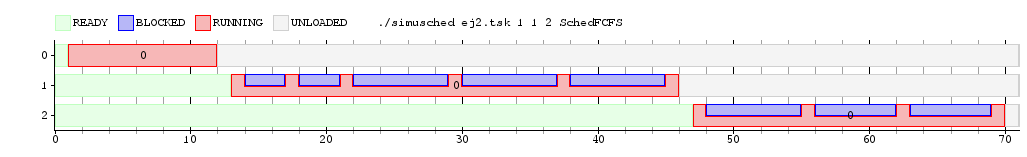
\includegraphics[scale=0.32]{images/ej2_1.png}
  \caption{Diagrama de Gantt para el lote 2 en FCFS con un n\'ucleo}
  \end{figure}
  \begin{figure}[htb]
  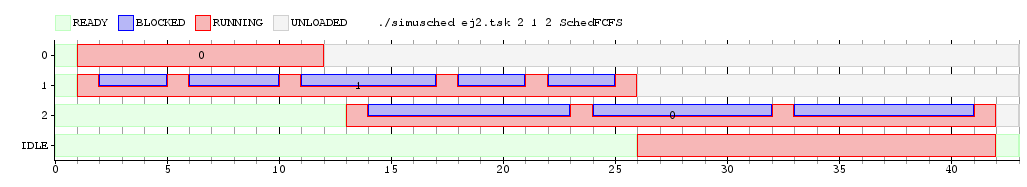
\includegraphics[scale=0.32]{images/ej2_2.png}
  \caption{Diagrama de Gantt para el lote 2 en FCFS con dos n\'ucleos}
  \end{figure}
  \begin{figure}[htb]
  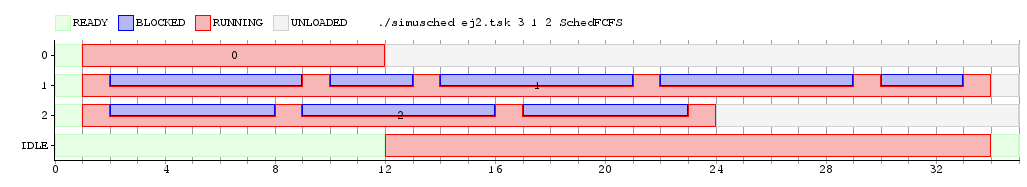
\includegraphics[scale=0.32]{images/ej2_3.png}
  \caption{Diagrama de Gantt para el lote 2 en FCFS con tres n\'ucleos}
  \end{figure}
